%%
%% Automatically generated file from DocOnce source
%% (https://github.com/hplgit/doconce/)
%%
%%
% #ifdef PTEX2TEX_EXPLANATION
%%
%% The file follows the ptex2tex extended LaTeX format, see
%% ptex2tex: http://code.google.com/p/ptex2tex/
%%
%% Run
%%      ptex2tex myfile
%% or
%%      doconce ptex2tex myfile
%%
%% to turn myfile.p.tex into an ordinary LaTeX file myfile.tex.
%% (The ptex2tex program: http://code.google.com/p/ptex2tex)
%% Many preprocess options can be added to ptex2tex or doconce ptex2tex
%%
%%      ptex2tex -DMINTED myfile
%%      doconce ptex2tex myfile envir=minted
%%
%% ptex2tex will typeset code environments according to a global or local
%% .ptex2tex.cfg configure file. doconce ptex2tex will typeset code
%% according to options on the command line (just type doconce ptex2tex to
%% see examples). If doconce ptex2tex has envir=minted, it enables the
%% minted style without needing -DMINTED.
% #endif

% #define PREAMBLE

% #ifdef PREAMBLE
%-------------------- begin preamble ----------------------

\documentclass[%
oneside,                 % oneside: electronic viewing, twoside: printing
final,                   % draft: marks overfull hboxes, figures with paths
10pt]{article}

\listfiles               %  print all files needed to compile this document

\usepackage{relsize,makeidx,color,setspace,amsmath,amsfonts,amssymb}
\usepackage[table]{xcolor}
\usepackage{bm,ltablex,microtype}

\usepackage[pdftex]{graphicx}

\usepackage{ptex2tex}
% #ifdef MINTED
\usepackage{minted}
\usemintedstyle{default}
% #endif

\usepackage[T1]{fontenc}
%\usepackage[latin1]{inputenc}
\usepackage{ucs}
\usepackage[utf8x]{inputenc}

\usepackage{lmodern}         % Latin Modern fonts derived from Computer Modern

% Hyperlinks in PDF:
\definecolor{linkcolor}{rgb}{0,0,0.4}
\usepackage{hyperref}
\hypersetup{
    breaklinks=true,
    colorlinks=true,
    linkcolor=linkcolor,
    urlcolor=linkcolor,
    citecolor=black,
    filecolor=black,
    %filecolor=blue,
    pdfmenubar=true,
    pdftoolbar=true,
    bookmarksdepth=3   % Uncomment (and tweak) for PDF bookmarks with more levels than the TOC
    }
%\hyperbaseurl{}   % hyperlinks are relative to this root

\setcounter{tocdepth}{2}  % levels in table of contents

% Tricks for having figures close to where they are defined:
% 1. define less restrictive rules for where to put figures
\setcounter{topnumber}{2}
\setcounter{bottomnumber}{2}
\setcounter{totalnumber}{4}
\renewcommand{\topfraction}{0.95}
\renewcommand{\bottomfraction}{0.95}
\renewcommand{\textfraction}{0}
\renewcommand{\floatpagefraction}{0.75}
% floatpagefraction must always be less than topfraction!
% 2. ensure all figures are flushed before next section
\usepackage[section]{placeins}
% 3. enable begin{figure}[H] (often leads to ugly pagebreaks)
%\usepackage{float}\restylefloat{figure}

\usepackage[framemethod=TikZ]{mdframed}

% --- begin definitions of admonition environments ---

% --- end of definitions of admonition environments ---

% prevent orhpans and widows
\clubpenalty = 10000
\widowpenalty = 10000

% --- end of standard preamble for documents ---


% insert custom LaTeX commands...

\raggedbottom
\makeindex
\usepackage[totoc]{idxlayout}   % for index in the toc
\usepackage[nottoc]{tocbibind}  % for references/bibliography in the toc

%-------------------- end preamble ----------------------

\begin{document}

% matching end for #ifdef PREAMBLE
% #endif

\newcommand{\exercisesection}[1]{\subsection*{#1}}


% ------------------- main content ----------------------



% ----------------- title -------------------------

\thispagestyle{empty}

\begin{center}
{\LARGE\bf
\begin{spacing}{1.25}
Modelli computazionali per la scuola superiore
\end{spacing}
}
\end{center}

% ----------------- author(s) -------------------------

\begin{center}
{\bf Morten Hjorth-Jensen${}^{1, 2}$} \\ [0mm]
\end{center}

\begin{center}
% List of all institutions:
\centerline{{\small ${}^1$Dipartimento di Fisica e \href{{http://www.mn.uio.no/ccse/english/people/index.html}}{Centro per Computing in Science Education}, Univ Oslo, Norvegia}}
\centerline{{\small ${}^2$Dipartimento di Fisica ed Astronomia, Michigan State University, USA}}
\end{center}
    
% ----------------- end author(s) -------------------------

% --- begin date ---
\begin{center}
Sep 12, 2017
\end{center}
% --- end date ---

\vspace{1cm}


% !split
\subsection{Unique opportunities}

% --- begin paragraph admon ---
\paragraph{}
Computing competence represents a central element
in scientific problem solving, from basic education and research to
essentially almost all advanced problems in modern
societies.

Computing competence \textbf{enlarges the body of tools available to students} and
scientists beyond classical tools and \textbf{allows for a more generic
handling of problems}. Focusing on algorithmic aspects \textbf{results in
deeper insights} about scientific problems.
% --- end paragraph admon ---





% !split
\subsection{Why is computing competence important?}
The impact of the computer on mathematics and science is tremendous: \textbf{science and industry now rely on solving mathematical problems through computing}.
\begin{itemize}
\item Computing can increase the relevance in education by solving more realistic problems earlier.

\item Computing through programming can be excellent training of creativity.

\item Computing can enhance the understanding of abstractions and generalization.

\item Computing can decrease the need for special tricks and tedious algebra, and shifts the focus to problem definition, visualization, and "what if" discussions.
\end{itemize}

\noindent
% !split
\subsection{Come introdurre metodi numerici nelle scuole superiori: Un modello per prede e predatori}


% --- begin paragraph admon ---
\paragraph{}
The population dynamics of a simple predator-prey system is a
classical example shown in many biology textbooks when ecological
systems are discussed. The system contains all elements of the
scientific method:

\begin{itemize}
 \item The set up of a specific hypothesis combined with

 \item the experimental methods needed (one can study existing data or perform experiments)

 \item analyzing and interpreting the data and performing further experiments if needed

 \item trying to extract general behaviors and extract eventual laws or patterns

 \item develop mathematical relations for the uncovered regularities/laws and test these by per forming new experiments
\end{itemize}

\noindent
% --- end paragraph admon ---




% !split
\subsection{Lepre e lince nella baia di Hudson}


% --- begin paragraph admon ---
\paragraph{}
Lots of data about populations of hares and lynx collected from furs in Hudson Bay, Canada, are available. It is known that the populations oscillate. Why?
We shall demonstrate the scientific method by

\begin{enumerate}
\item plotting the data

\item derive a simple model for the population dynamics

\item (fitting parameters in the model to the data)

\item using the model predict the evolution other predator-pray systems
\end{enumerate}

\noindent
% --- end paragraph admon ---



% !split
\subsection{Hudson bay data}



% --- begin paragraph admon ---
\paragraph{}


\begin{quote}
\begin{tabular}{lrr}
\hline
\multicolumn{1}{c}{ Anno } & \multicolumn{1}{c}{ Lepri (x1000) } & \multicolumn{1}{c}{ Linci (x1000) } \\
\hline
1900 & 30.0          & 4.0           \\
1901 & 47.2          & 6.1           \\
1902 & 70.2          & 9.8           \\
1903 & 77.4          & 35.2          \\
1904 & 36.3          & 59.4          \\
1905 & 20.6          & 41.7          \\
1906 & 18.1          & 19.0          \\
1907 & 21.4          & 13.0          \\
1908 & 22.0          & 8.3           \\
1909 & 25.4          & 9.1           \\
1910 & 27.1          & 7.4           \\
1911 & 40.3          & 8.0           \\
1912 & 57            & 12.3          \\
1913 & 76.6          & 19.5          \\
1914 & 52.3          & 45.7          \\
1915 & 19.5          & 51.1          \\
1916 & 11.2          & 29.7          \\
1917 & 7.6           & 15.8          \\
1918 & 14.6          & 9.7           \\
1919 & 16.2          & 10.1          \\
1920 & 24.7          & 8.6           \\
\hline
\end{tabular}
\end{quote}

\noindent
% --- end paragraph admon ---





% !split
\subsection{Plotting the data}


% --- begin paragraph admon ---
\paragraph{}
\bpypro
import numpy as np
from  matplotlib import pyplot as plt

# Load in data file
data = np.loadtxt('Hudson_Bay.dat', delimiter=',', skiprows=1)
# Make arrays containing x-axis and hares and lynx populations
year = data[:,0]
hares = data[:,1]
lynx = data[:,2]

plt.plot(year, hares ,'b-+', year, lynx, 'r-o')
plt.axis([1900,1920,0, 100.0])
plt.xlabel(r'Year')
plt.ylabel(r'Numbers of hares and lynx ')
plt.legend(('Hares','Lynx'), loc='upper right')
plt.title(r'Population of hares and lynx from 1900-1920 (x1000)}')
plt.savefig('Hudson_Bay_data.pdf')
plt.savefig('Hudson_Bay_data.png')
plt.show()
\epypro
% --- end paragraph admon ---



% !split
\subsection{Hares and lynx in Hudson bay from 1900 to 1920}



\vspace{6mm}

% inline figure
\centerline{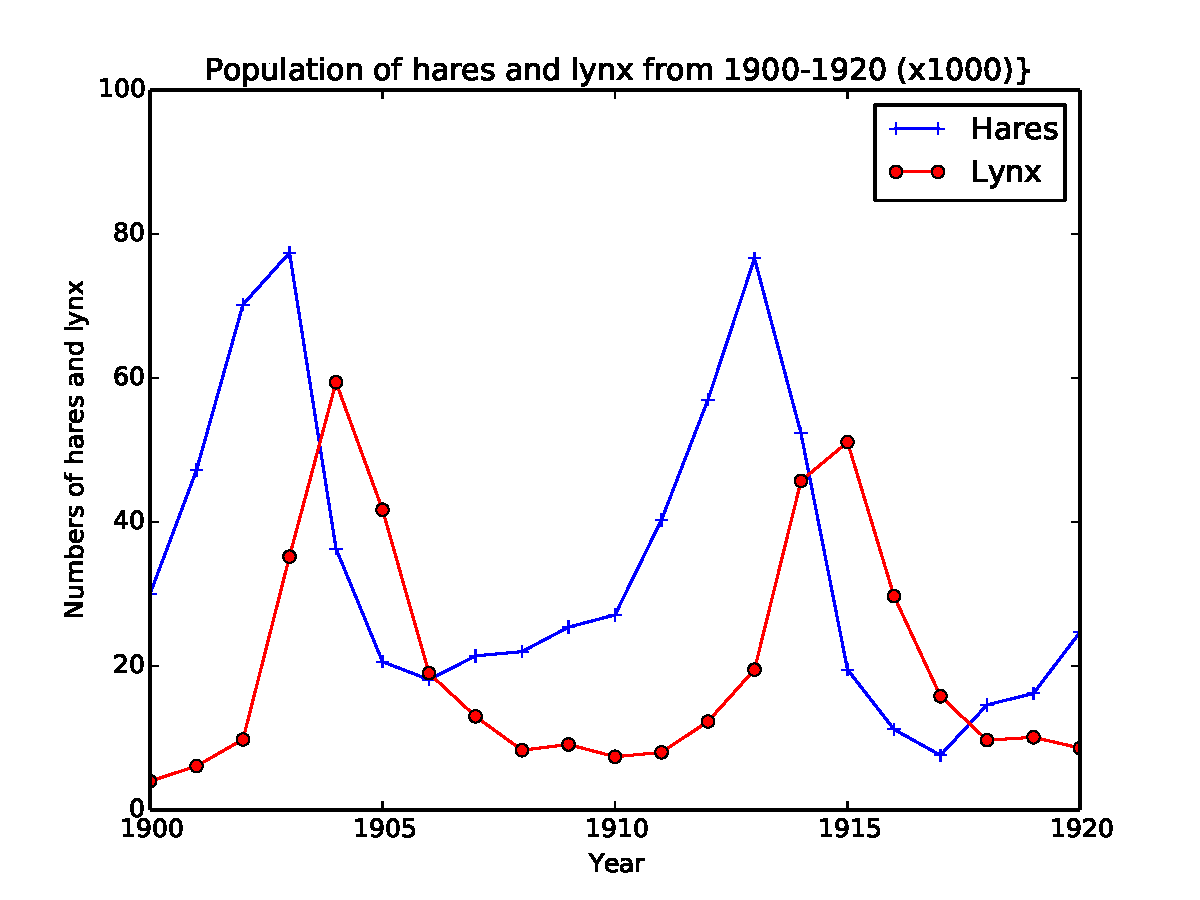
\includegraphics[width=0.9\linewidth]{fig/Hudson_Bay_data.pdf}}

\vspace{6mm}




% !split
\subsection{Why now create a computer model for the hare and lynx populations?}

% --- begin paragraph admon ---
\paragraph{}
\begin{itemize}
 \item We see oscillations in the data

 \item What causes cycles to slow or speed up?

 \item What affects the amplitude of the oscillation or do you expect to see the oscillations damp to a stable equilibrium?

 \item With a model we can better \emph{understand the data}

 \item More important: we can understand the ecology dynamics of
   predator-pray populations
\end{itemize}

\noindent
% --- end paragraph admon ---




% !split
\subsection{The traditional (top-down) approach}


% --- begin paragraph admon ---
\paragraph{}
The classical way (in all books) is to present the Lotka-Volterra equations:

\begin{align*}
\frac{dH}{dt} &= H(a - b L)\\ 
\frac{dL}{dt} &= - L(d - c  H)
\end{align*}

Here,

\begin{itemize}
 \item $H$ is the number of preys

 \item $L$ the number of predators

 \item $a$, $b$, $d$, $c$ are parameters
\end{itemize}

\noindent
Most books quickly establish the model and then use considerable space on
discussing the qualitative properties of this \emph{nonlinear system of
ordinary differential equations} (which cannot be solved analytically)
% --- end paragraph admon ---




% !split
\subsection{The ``new'' discrete bottom-up approach}


% --- begin paragraph admon ---
\paragraph{The bottom-up approach.}
% !bpop
\begin{itemize}
 \item Start with experimental data and discuss the methods which have been used to collect the data, the assumptions, the electronic devices, the aims etc. That is, expose the students to the theory and assumptions behind the data that have been collected and motivate for the scientific method.

 \item Where appropriate the students should do the experiment(s) needed to collect the data.

 \item The first programming tasks are to read and visualize the data to see if there are patterns or regularities. This strengthens a research-driven intuition.

 \item Now we want to increase the understanding through modeling.

 \item Most of the biology lies in the \emph{derivation} of the model. We shall
   focus on an intuitive discrete approach that leads to difference
   equations that can be programmed \emph{and solved} directly.
\end{itemize}

\noindent
% !epop
% --- end paragraph admon ---



% !split
\subsection{Basic (computer-friendly) mathematics notation}

% --- begin paragraph admon ---
\paragraph{}
\begin{itemize}
 \item Time points: $t_0,t_1,\ldots,t_m$

 \item Uniform distribution of time points: $t_n=n\Delta t$

 \item $H^n$: population of hares at time $t_n$

 \item $L^n$: population of lynx at time $t_n$

 \item We want to model the changes in populations, $\Delta H=H^{n+1}-H^n$
   and $\Delta L=L^{n+1}-L^n$ during a general time interval $[t_{n+1},t_n]$
   of length $\Delta t=t_{n+1}-t_n$
\end{itemize}

\noindent
% --- end paragraph admon ---



% !split
\subsection{Basic dynamics of the population of hares, vita e morte}


% --- begin paragraph admon ---
\paragraph{}
The population of hares evolves due to births and deaths

\[
\Delta H = a \Delta t H^n
\]
However, hares have an additional loss in the population because
they are eaten by lynx.
All the hares and lynx can form
$H\cdot L$ pairs in total. When such pairs meet during a time
interval $\Delta t$, there is some
small probablity that the lynx will eat the hare.
So in fraction $b\Delta t HL$, the lynx eat hares. This
loss of hares and must be accounted for:
subtracted in the equation for hares:

\[ \Delta H = a\Delta t H^n - b \Delta t H^nL^n\]
% --- end paragraph admon ---



% !split
\subsection{Basic dynamics of the population of lynx}


% --- begin paragraph admon ---
\paragraph{}
We assume that the primary growth for the lynx population depends on sufficient food for raising lynx kittens, which implies an adequate source of nutrients from predation on hares. Thus, the growth of the lynx population does not only depend of how many lynx there are, but on how many hares they can eat.
In a time interval $\Delta t HL$ hares and lynx can meet, and in a
fraction $b\Delta t HL$ the lynx eats the hare. All of this does not
contribute to the growth of lynx, again just a fraction of
$b\Delta t HL$ that we write as
$d\Delta t HL$. In addition, lynx die just as in the population
dynamics with one isolated animal population, leading to a loss
$-c\Delta t L$.
% --- end paragraph admon ---




% --- begin paragraph admon ---
\paragraph{}
The accounting of lynx then looks like
\[ \Delta L = d\Delta t H^nL^n - c\Delta t L^n\]
% --- end paragraph admon ---



% !split
\subsection{Evolution equations}


% --- begin paragraph admon ---
\paragraph{}
By writing up the definition of $\Delta H$ and $\Delta L$, and putting
all assumed known terms $H^n$ and $L^n$ on the right-hand side, we have

\[ H^{n+1} = H^n + a\Delta t H^n - b\Delta t H^n L^n \]

\[ L^{n+1} = L^n + d\Delta t H^nL^n - c\Delta t L^n \]

Note:

\begin{itemize}
 \item These equations are ready to be implemented!

 \item But to start, we need $H^0$ and $L^0$ \\
   (which we can get from the data)

 \item We also need values for $a$, $b$, $d$, $c$
\end{itemize}

\noindent
% --- end paragraph admon ---



% !split
\subsection{Adapt the model to the Hudson Bay case}


% --- begin paragraph admon ---
\paragraph{}
\begin{itemize}
 \item As always, models tend to be general - as here, applicable
   to ``all'' predator-pray systems

 \item The critical issue is whether the \emph{interaction} between hares and lynx
   is sufficiently well modeled by $\hbox{const}HL$

 \item The parameters $a$, $b$, $d$, and $c$ must be
   estimated from data

 \item Measure time in years

 \item $t_0=1900$, $t_m=1920$
\end{itemize}

\noindent
% --- end paragraph admon ---



% !split
\subsection{The program}


% --- begin paragraph admon ---
\paragraph{}
\bpypro
import numpy as np
import matplotlib.pyplot as plt

def solver(m, H0, L0, dt, a, b, c, d, t0):
    """Solve the difference equations for H and L over m years
    with time step dt (measured in years."""

    num_intervals = int(m/float(dt))
    t = np.linspace(t0, t0 + m, num_intervals+1)
    H = np.zeros(t.size)
    L = np.zeros(t.size)

    print 'Init:', H0, L0, dt
    H[0] = H0
    L[0] = L0

    for n in range(0, len(t)-1):
        H[n+1] = H[n] + a*dt*H[n] - b*dt*H[n]*L[n]
        L[n+1] = L[n] + d*dt*H[n]*L[n] - c*dt*L[n]
    return H, L, t

# Load in data file
data = np.loadtxt('Hudson_Bay.csv', delimiter=',', skiprows=1)
# Make arrays containing x-axis and hares and lynx populations
t_e = data[:,0]
H_e = data[:,1]
L_e = data[:,2]

# Simulate using the model
H, L, t = solver(m=20, H0=34.91, L0=3.857, dt=0.1,
                 a=0.4807, b=0.02482, c=0.9272, d=0.02756,
                 t0=1900)

# Visualize simulations and data
plt.plot(t_e, H_e, 'b-+', t_e, L_e, 'r-o', t, H, 'm--', t, L, 'k--')
plt.xlabel('Year')
plt.ylabel('Numbers of hares and lynx')
plt.axis([1900, 1920, 0, 140])
plt.title(r'Population of hares and lynx 1900-1920 (x1000)')
plt.legend(('H_e', 'L_e', 'H', 'L'), loc='upper left')
plt.savefig('Hudson_Bay_sim.pdf')
plt.savefig('Hudson_Bay_sim.png')
plt.show()
\epypro
% --- end paragraph admon ---



% !split
\subsection{The plot}



\vspace{6mm}

% inline figure
\centerline{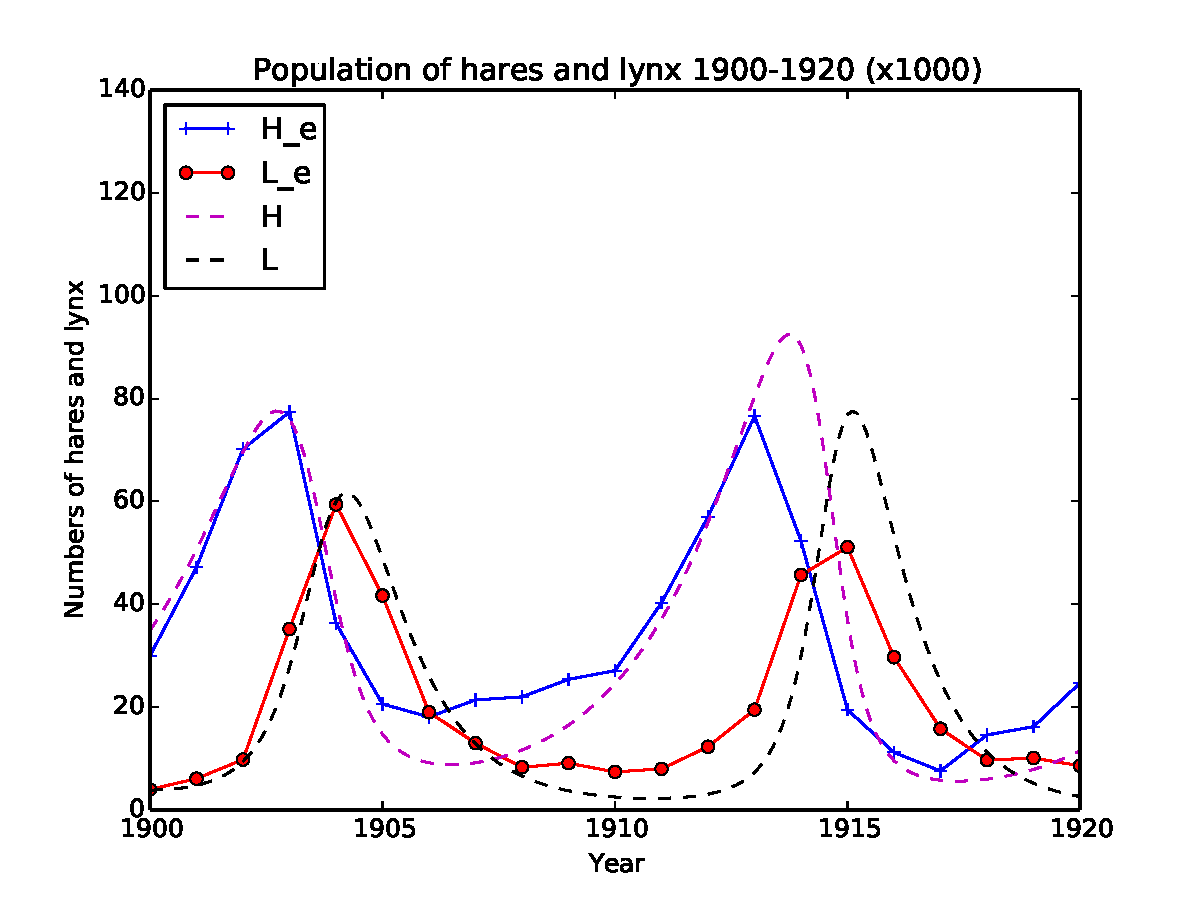
\includegraphics[width=0.9\linewidth]{fig/Hudson_Bay_sim.pdf}}

\vspace{6mm}




% !split
\subsection{Le equazioni di Newton con forze gravitazionali}

% --- begin paragraph admon ---
\paragraph{}
\bpycod
import numpy as np
from math import *
import matplotlib.pyplot as plt

def solver(m, dt, t0):
    """Solve the difference equations for H and L over m years
    with time step dt (measured in years."""

    num_intervals = int(m/float(dt))
    t = np.linspace(t0, t0 + m, num_intervals+1)
    x = np.zeros(t.size)
    y = np.zeros(t.size)
    vx = np.zeros(t.size)
    vy = np.zeros(t.size)
    r = np.zeros(t.size)
    v = np.zeros(t.size)


    x[0] = 1.0
    y[0] = 0.0
    vx[0] = 2.0*pi
    vy[0] = 0.0
    pi4 = 4.0*pi*pi
    for n in range(0, len(t)-1):
        x[n+1] = x[n] + dt*vx[n]
        y[n+1] = y[n] + dt*vy[n]
        r3 = (x[n]*x[n]+y[n]*y[n])**3
        vx[n+1] = vx[n] -dt*pi4*x[n]/r3
        vy[n+1] = vy[n] -dt*pi4*y[n]/r3
        v[n+1] = sqrt(vx[n+1]*vx[n+1]+vy[n+1]*vy[n+1])
        r[n+1] = sqrt(x[n+1]*x[n+1]+y[n+1]*y[n+1])

    return r, v, t
# Simulate using the model
m =20 # 20 years
dt =0.01 # stepsize
t0 =0.0
r, v, t = solver(m, dt,t0)
# Visualize simulations and data
plt.plot(r, v, 'b-+')
plt.xlabel('r')
plt.ylabel('velocity')
plt.axis([0, 2.0, 0, 4*pi])
plt.title(r'Velocity versus position')
plt.savefig('SunEarth.pdf')
plt.show()

\epycod
% --- end paragraph admon ---








% ------------------- end of main content ---------------

% #ifdef PREAMBLE
\end{document}
% #endif

